\documentclass[a4paper,11pt]{article}


\usepackage[latin1]{inputenc}
\usepackage{color}
\usepackage{array}
\usepackage[Spanish]{babel}
\usepackage{amsmath,amssymb}
\usepackage{graphicx}
\usepackage{ragged2e}
\usepackage{multicol}

\addtolength{\textwidth}{2cm}
\addtolength{\hoffset}{-1cm}




\title{``Python''}
\author{Tania S\'{a}nchez\\ Marlon Loayza}

\begin{document}

\setlength{\topmargin}{0.5in}
			\pagestyle{empty}
			\begin{center}
				\textbf{
					\vspace{-0.7em}
					ESCUELA SUPERIOR POLIT\'{E}CNICA DEL LITORAL
				}
				\line(1,0){380}\\		
				\scriptsize{FACULTAD DE INGENIER\'{I}A EN ELECTRICIDAD Y COMPUTACI\'{O}N}
				
				\vspace{2.5em}
				
\includegraphics[scale=0.2]{images/logo_espol.jpg} 
			\end{center}
			
			\begin{center}
				\vspace{2.5em}
				Lenguajes de Programaci\'{o}n
				\\II T\'{e}rmino - 2012
				\vspace{1.5em}  %espacio entre linea anterior y la siguiente
				\\Manual de Usuario \\Proyecto Python\\
				\vspace{5em}
				\Huge{\textbf{``Quien Sabe Sabe!!...''	\vspace{3em}}}
			\end{center}	
			
			


				\hspace*{5cm}Desarrolladores:
				\vspace{1.5em}
				\\\hspace*{8cm}Tania S\'{a}nchez
				\\\hspace*{8cm}Marlon Loayza 


\newpage 

\setlength{\topmargin}{-0,2in}
\tableofcontents

\newpage 

\section{Introducci\'{o}n}
El presente manual ha sido creado para facilitar el uso del programa {\textbf{\textit{``QUIEN SABE, SABE!!!''}}, que es un juego elaborado en lenguaje Python, como proyecto de la materia de Lenguajes de Programaci\'{o}n en el a\~{n}o 2012, II t\'{e}rmino.
\newline
\newline
Este es un programa de concursos basado en el formato de preguntas y respuestas del \textbf{juego quien quiere ser millonario}, que ofrece grandes premios monetarios por responder correctamente a una serie de preguntas de opci\'{o}n m\'{u}ltiple con dificultad creciente.  
\newline
\newline
\section{La aplicaci\'{o}n}

\subsection{Nombre y Descripci\'{o}n del Proyecto}
\vspace{1.5em}
 \centerline{\textbf{\textit{ ``QUIEN SABE, SABE!!!''}}}
\vspace{1.5em}
Este juego consta de preguntas que ofrecen cuatro posibles respuestas, se dan (A, B, C o D), y el concursante debe elegir la correcta. En respuesta a la primera pregunta contestada correctamente, el concursante gana \$ 200 (Americanos). En esta versi\'{o}n no hay l\'{i}mite de tiempo para responder a una pregunta, un jugador puede (y a menudo lo hace) tomar el tiempo que necesita para reflexionar sobre una respuesta a escoger.
\newline
\newline
Para preguntas posteriores se juega por sumas cada vez m\'{a}s grandes (m\'{a}s o menos duplicar en cada vuelta). Las primeras preguntas suelen tener algunas respuestas broma. La secuencia completa de puntos para esta versi\'{o}n es la siguiente:
\newline



\begin{multicols}{2}
	\begin{itemize}
		\item \$ 200
		\item \$ 300
		\item \$ 500
		\item \$ 1000
		\item \$ 2000
		\item \$ 4000
		\item \$ 8000
		\item \$ 16000
		\item \$ 32000
		\item \$ 64000
		\item \$ 125000
		\item \$ 250000
		\item \$ 500000
		\item \$ 1000000
	\end{itemize}
\end{multicols}

\subsection{Funcionalidades}

\textbf{\textit{``QUIEN SABE, SABE!!!''}} es un juego pensado para personas con deficiencia visual cuenta con un men\'{u} inicio donde cada opci\'{o}n fue grabada por medio de un programa llamado \textbf{\textit{``BALABOLKA''}}, estas grabaciones fueron llamadas en el c\'{o}digo del juego para poderlas escuchar al ejecutarlo.\\ \\Las opciones del men\'{u} inicial son las siguientes: 

	\begin{itemize}
		\item Jugar,
		\item Instrucciones,
		\item Autores y 
		\item Salir.
	\end{itemize}
Estas opciones pueden ser escogidas presionando la primera letra de cada palabra como lo dice el juego siendo asi, si queremos escoger la opci\'{o}n \textbf{\textit{``Jugar''}} se deber\'{a} presionar la tecla \textbf{\textit{``J''}}, si se desea la opci\'{o}n \textbf{\textit{``Instrucciones''}} presionaremos la tecla \textbf{\textit{``I''}} y as\'{i} con cada opci\'{o}n a escoger.
\begin{center}
	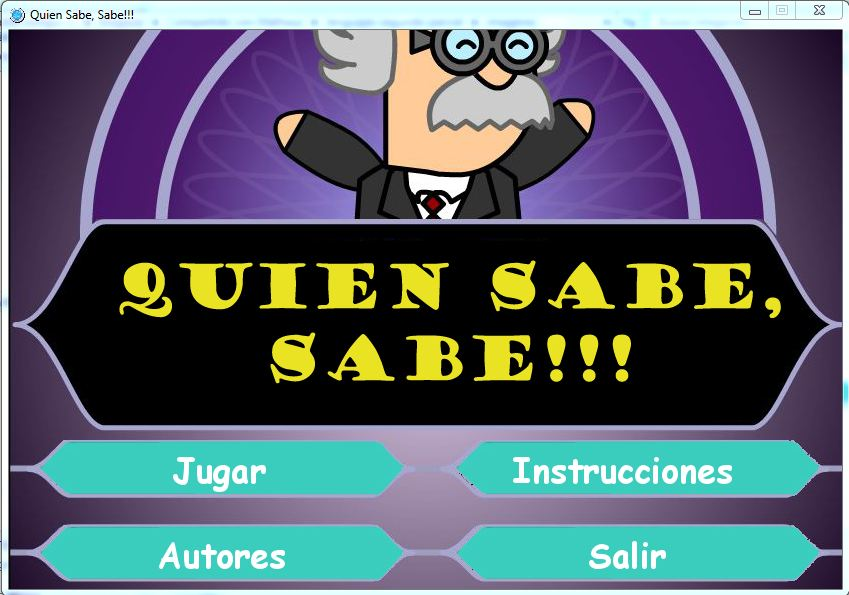
\includegraphics[scale=0.5]{images/inicio.JPG} 
\end{center}
	
\subsubsection{Jugar}

Al presionar el bot\'{o}n \textbf{``Jugar''} se muestra y se escucha la primera pregunta con sus cuatro opciones para contestarla, si el jugador escoge la opcion correcta el puntaje o score aumentar\'{a} y proceder\'{a} a mostrar y decir la segunda pregunta con sus respectivas opciones y asi hasta contestar las quince preguntas, si el jugador contesta de manera incorrecta automaticamente perder\'{a} el juego y se regresar\'{a} al menu inicial.
\\
Las opciones de respuesta est\'{a}n clasificadas en (A,B,C,D) facilitando al jugador poder escoger la respuesta deseada siendo as\'{i} si el jugador considera que la respuesta correcta es la del literal A presionar\'{a} la \textbf{tecla A}, si cree que es la del literal B deber\'{a} presionar la \textbf{tecla B}, si cree que es la C presionar\'{a} la \textbf{tecla C} caso contrario presionar\'{a} la \textbf{tecla D} esto ser\'{a} seg\'{u}n su criterio o conocimiento.
	\begin{center}
		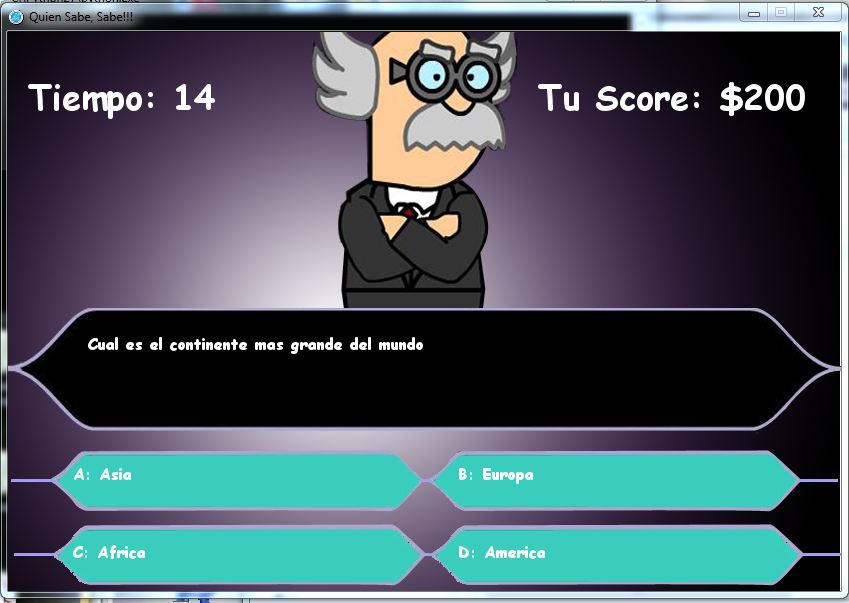
\includegraphics[scale=0.5]{images/jugando1.jpg}
	\end{center}
	
\subsubsection{Instrucciones}
	
	El bot\'{o}n de \textbf{``Instrucciones''} como su nombre lo dice nos facilita las instrucciones del juego.
		\newline

		\begin{center}
			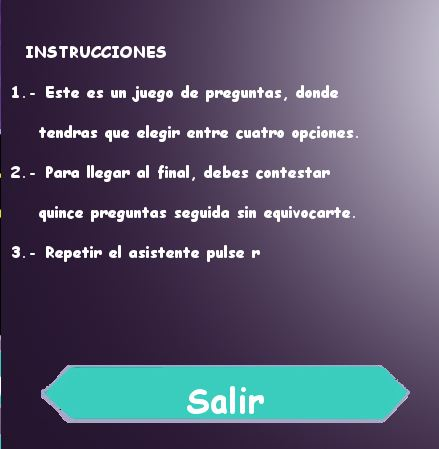
\includegraphics[scale=0.6]{images/instrucciones.jpg}
		\end{center}
	
		
\newpage

\subsubsection{Autores}

			El bot\'{o}n \textbf{``Autores''} permitir\'{a} conocer a los desarrolladores del programa \textbf{``QUIEN SABE, SABE!!!''} y tambi\'{e}n un link de referencia de donde se obtuvo la idea del juego.
			
	\begin{center}
		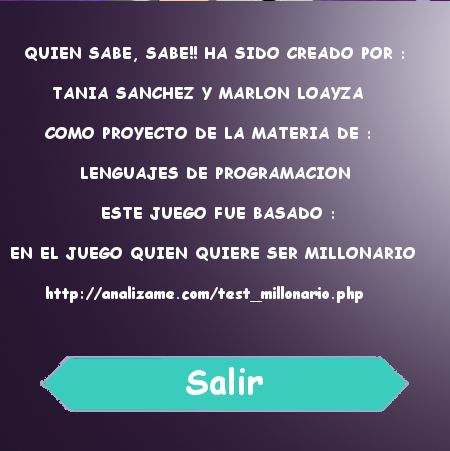
\includegraphics[scale=0.6]{images/autores.jpg} 
	\end{center}
		
		
\subsubsection{Salir}

		El bot\'{o}n \textbf{``Salir''} est\'{a} en caso de que se haya entrado por error o simplemente ya no se quiera seguir jugando.
		\newline



\newpage

\addcontentsline{toc}{section}{Referencias}
\begin{thebibliography}{99}

\bibitem{unistan}http://analizame.com/test\_millonario.php
\bibitem{acp} http://es.wikipedia.org/wiki/?`Qui\'{e}n\_quiere\_ser\_millonario\%3F.
\end{thebibliography}


\end{document}
